\documentclass[../diplomski_rad.tex]{subfiles}

\begin{document}

\sloppy

\justifying

Laboratorijska mjerenja provedena su u SleepdB laboratoriju (KITE Toronto Rehabilitation Institute, 
University Health Network, Toronto, Kanada). 
Istraživanje je odobrio Odbor za etičko istraživanje (University Health Network Research Ethics Board) (REB 18 5090). 
Svi ispitanici dali su pisani pristanak prije sudjelovanja u istraživanju. 
U istraživanju je sudjelovalo šest ispitanika čiji demografski podaci su prikazani u tablici \ref{tab:opci_podaci}, 
a mjerenja su provedena korištenjem razvijenog mjernog sustava (Slika X) 
i ranije opisanog SFB7 ImpediMed sustava \cite{sfb7}, koji se smatra zlatnim standardom. 
Također, uspoređeni su rezultati mjerenja dobiveni gel elektrodama s onima dobivenim tekstilnim elektrodama. 
Mjerni sustav je prikazan slikom X, gdje su vidljivi svi prethodno opisani dijelovi mjernog sustava.

\begin{table}[H]
\centering
\begin{tblr}{
    width=1\linewidth,
    cells={valign=m,halign=c},
    row{1}={bg=lightgray,font=\bfseries,rowsep=8pt},
    hlines,
    vlines
}
    \hline
    Broj ispitanika & Dob (godina) & Visina (cm) & Težina (kg) & BMI \\ [0.5ex] 
    \hline\hline
    6 & 26±5.44  & 174.16±12.09 & 74±15.61 & 24.28±3.65 \\
    \hline
\end{tblr}
\caption{\label{tab:opci_podaci}Demografski podaci}
\end{table}
    
Zbog svoje praktičnosti, udobnosti i kompatibilnosti, tekstilne elektrode sve više se integriraju u pametna nosiva 
rješenja kao preferirani izbor za praćenje zdravstvenih parametara, uključujući distribuciju tekućine \cite{Meding2021}. 
Tekstilne elektrode korištene u ovom radu nude neinvazivno i nosivo rješenje, omogućujući dugotrajno praćenje tekućine, 
posebno kod osoba sa srčanim zatajenjem \cite{McDonald2010},\cite{Gudmundsson2016}. 
Korištene su tekstilne elektrode razvijene unutar SleepdB istraživačke grupe \cite{Piper2023}. 
Tekstilne elektrode se temelje na vodljivom srebrenom materijalu, prikazane na slici \ref{slk:tekstilne_elektrode}, 
a koje su posebno dizajnirane za praćenje tekućine.

\begin{figure}[htb]
    \centering
    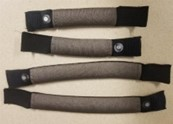
\includegraphics[width=0.45\textwidth]{Figures/tekstilne_elektrode.jpg} 
    \caption{Trake s tekstilnim elektrodama na bazi srebra koje pokrivaju cijeli opseg za praćenje tekućine \cite{Bandur2023}}
    \label{slk:tekstilne_elektrode}
\end{figure}

\section{Protokol mjerenja}

Razvijeni nosivi bežični sustav mjeri bioimpedanciju te izmjerene podatke BLE komunikacijskim protokolom šalje na udaljenu desktop aplikaciju. 
Aplikacija obavlja daljnje izračune volumena tekućine u tijelu i nogama. 
Korištena su dobivena mjerenja impedancije tijela za izračun volumena tekućine u tijelu koristeći MF BIA funkcije opisane u \cite{Sanchez2013}. 
Za izračun volumena tekućine u nozi, korištene su funkcije opisane u \cite{Delano2022}.

Za validaciju ispravnosti rada mjernog sustava provedena je vježba plantarne fleksija, 
prikazana na slici \ref{slk:plantarna_fleksija}, gdje je pozicija A neutralni položaj, 
gdje je stopalo ravno na tlu, a pozicija B je plantarna fleksija, gdje je stopalo usmjereno prema dolje. 
Plantarna fleksija u ovom radu koristi se za validaciju promjene tekućine u nogama jer aktivira 
mišiće gastrocnemius i soleus, što može potaknuti cirkulaciju krvi i limfne tekućine. 
Tijekom ove vježbe, pritisak na poplitealnu venu može poslužiti kao indikacija promjena u volumenu tekućine. 
Stoga, praćenje plantarne fleksije može pružiti vrijedne podatke o dinamici tekućine u donjim ekstremitetima, 
što je posebno korisno za pacijente sa srčanim zatajenjem ili drugim sličnim stanjima \cite{AVILADEOLIVEIRA2022102625}. 

\begin{figure}[htb]
    \centering
    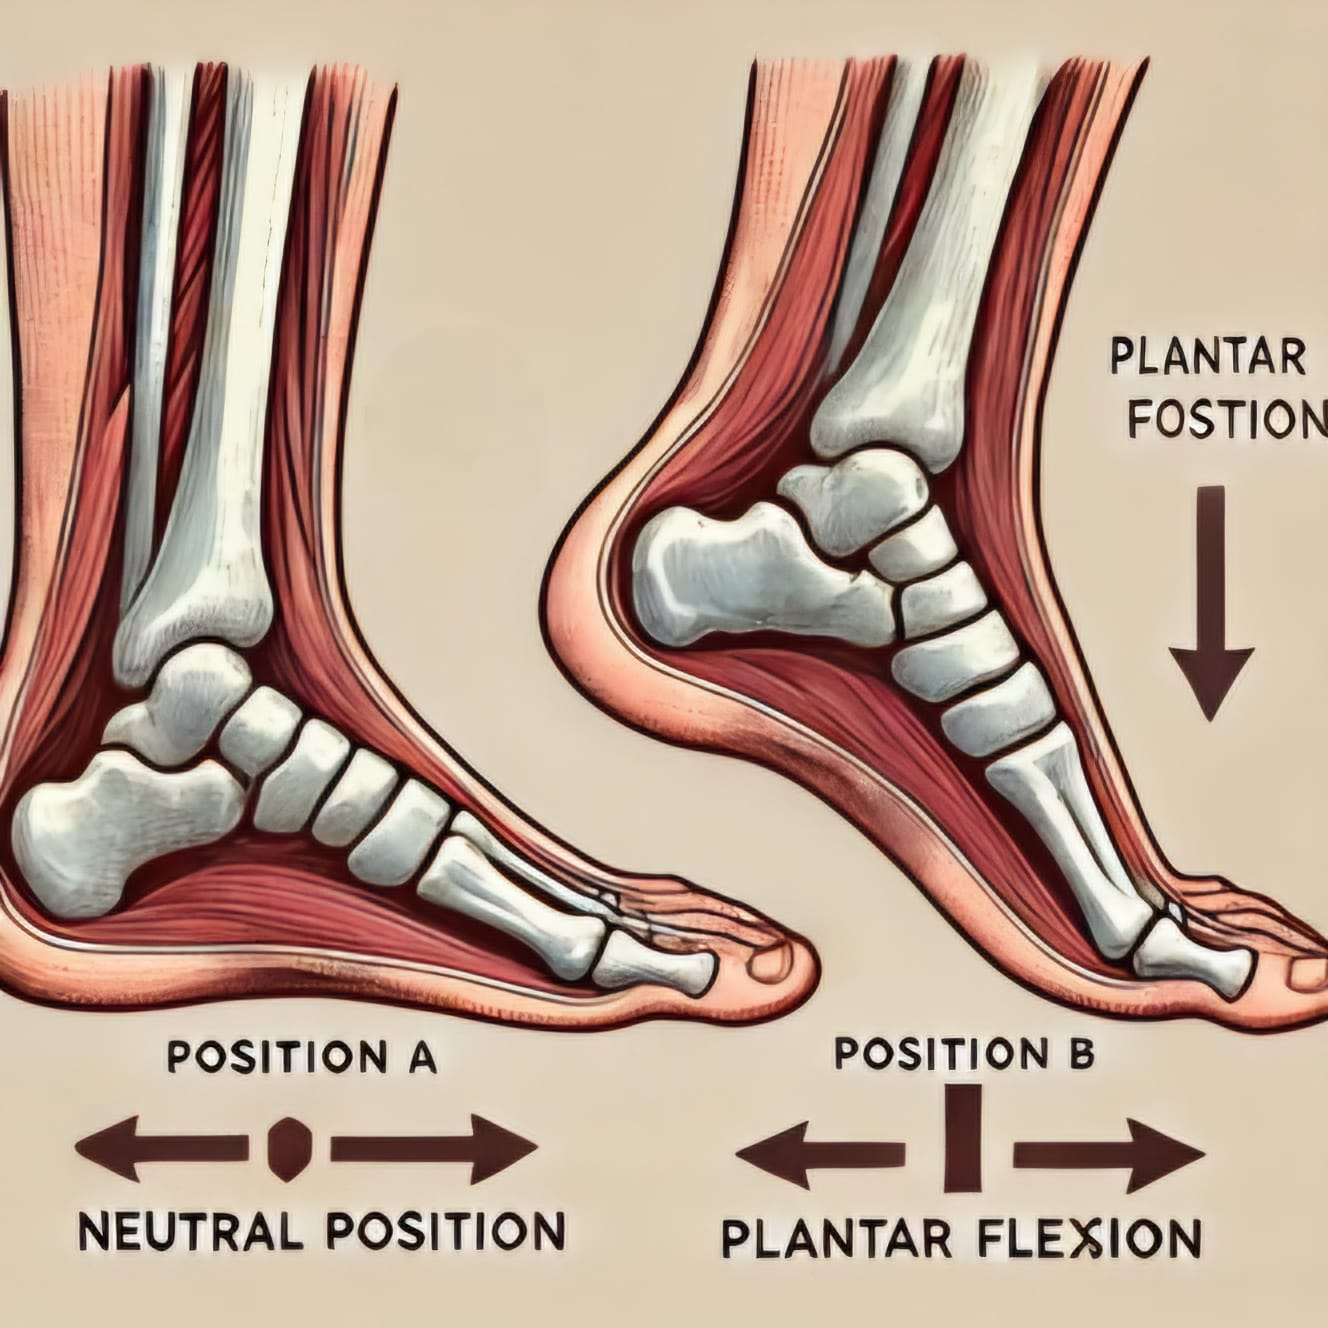
\includegraphics[width=0.45\textwidth]{Figures/plantarna_fleksija.jpg} 
    \caption{Ilustracija prikazuje neutralnu poziciju (A) i plantarnu fleksiju (B) stopala \newline (generirano pomoću DALL-E alata iz OpenAI)
    }
    \label{slk:plantarna_fleksija}
\end{figure}

U radu je provedeno kontinuirano ponavljanje pokreta plantarne fleksije pet minuta prema slici \ref{slk:protokol}, 
kako bi se odredilo učinkovita procjena promjene volumena tekućine u nogama. 

\begin{figure}[htb]
    \centering
    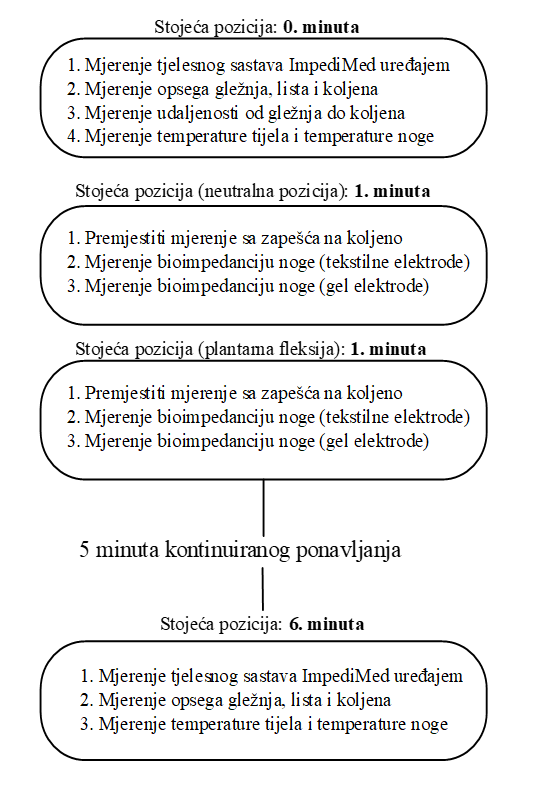
\includegraphics[width=0.65\textwidth]{Figures/protokol.png} 
    \caption{Protokol provedenih mjerenja}
    \label{slk:protokol}
\end{figure}

Hipoteza je da bi kontinuirano ponavljanje pokreta tijekom 5 minuta bilo učinkovitije u promjeni volumena 
tekućine u nogama u usporedbi s povremenim ponavljanjem pokreta s pauzama. 
Kontinuirana kontrakcija mišića osigurava stalni pritisak na poplitealnu venu, 
što bi trebalo rezultirati bržim smanjenjem tekućine u nogama zbog povećanog venskog povratka.

Tijekom mjerenja, na desnu potkoljenicu ispitanika postavljene su gel elektrode na istoj razini kao i 
tekstilne elektrode kako bi se osiguralo prikupljanje podataka s istog dijela tijela. 
Početno mjerenje cjelokupnog sastava tijela obavljeno je pomoću ImpediMed SFB7 dok je ispitanik bio u stojećem položaju. 
Mjerenje je dobiveno postavljanjem elektroda na zapešće desne ruke i gležanj desne noge. 
Za analizu impedancije noge, elektrode su bile postavljene na koljeno i gležanj desne noge.

Gel i tekstilne elektrode postavljene su na istoj visini na desnoj nozi sudionika, osiguravajući da se 
vodljivi tekstil ne preklapa s gel elektrodom \cite{Piper2023}. 
Elektrode su postavljene s minimalnim razmakom od 2 cm između parova. 
Također, za svakog ispitanika izmjeren je opseg oko koljena, gležnja i najšireg dijela lista, 
kao i udaljenost između dviju senzorskih (V+ i V-) elektroda.

\begin{figure}[htb]
    \centering
    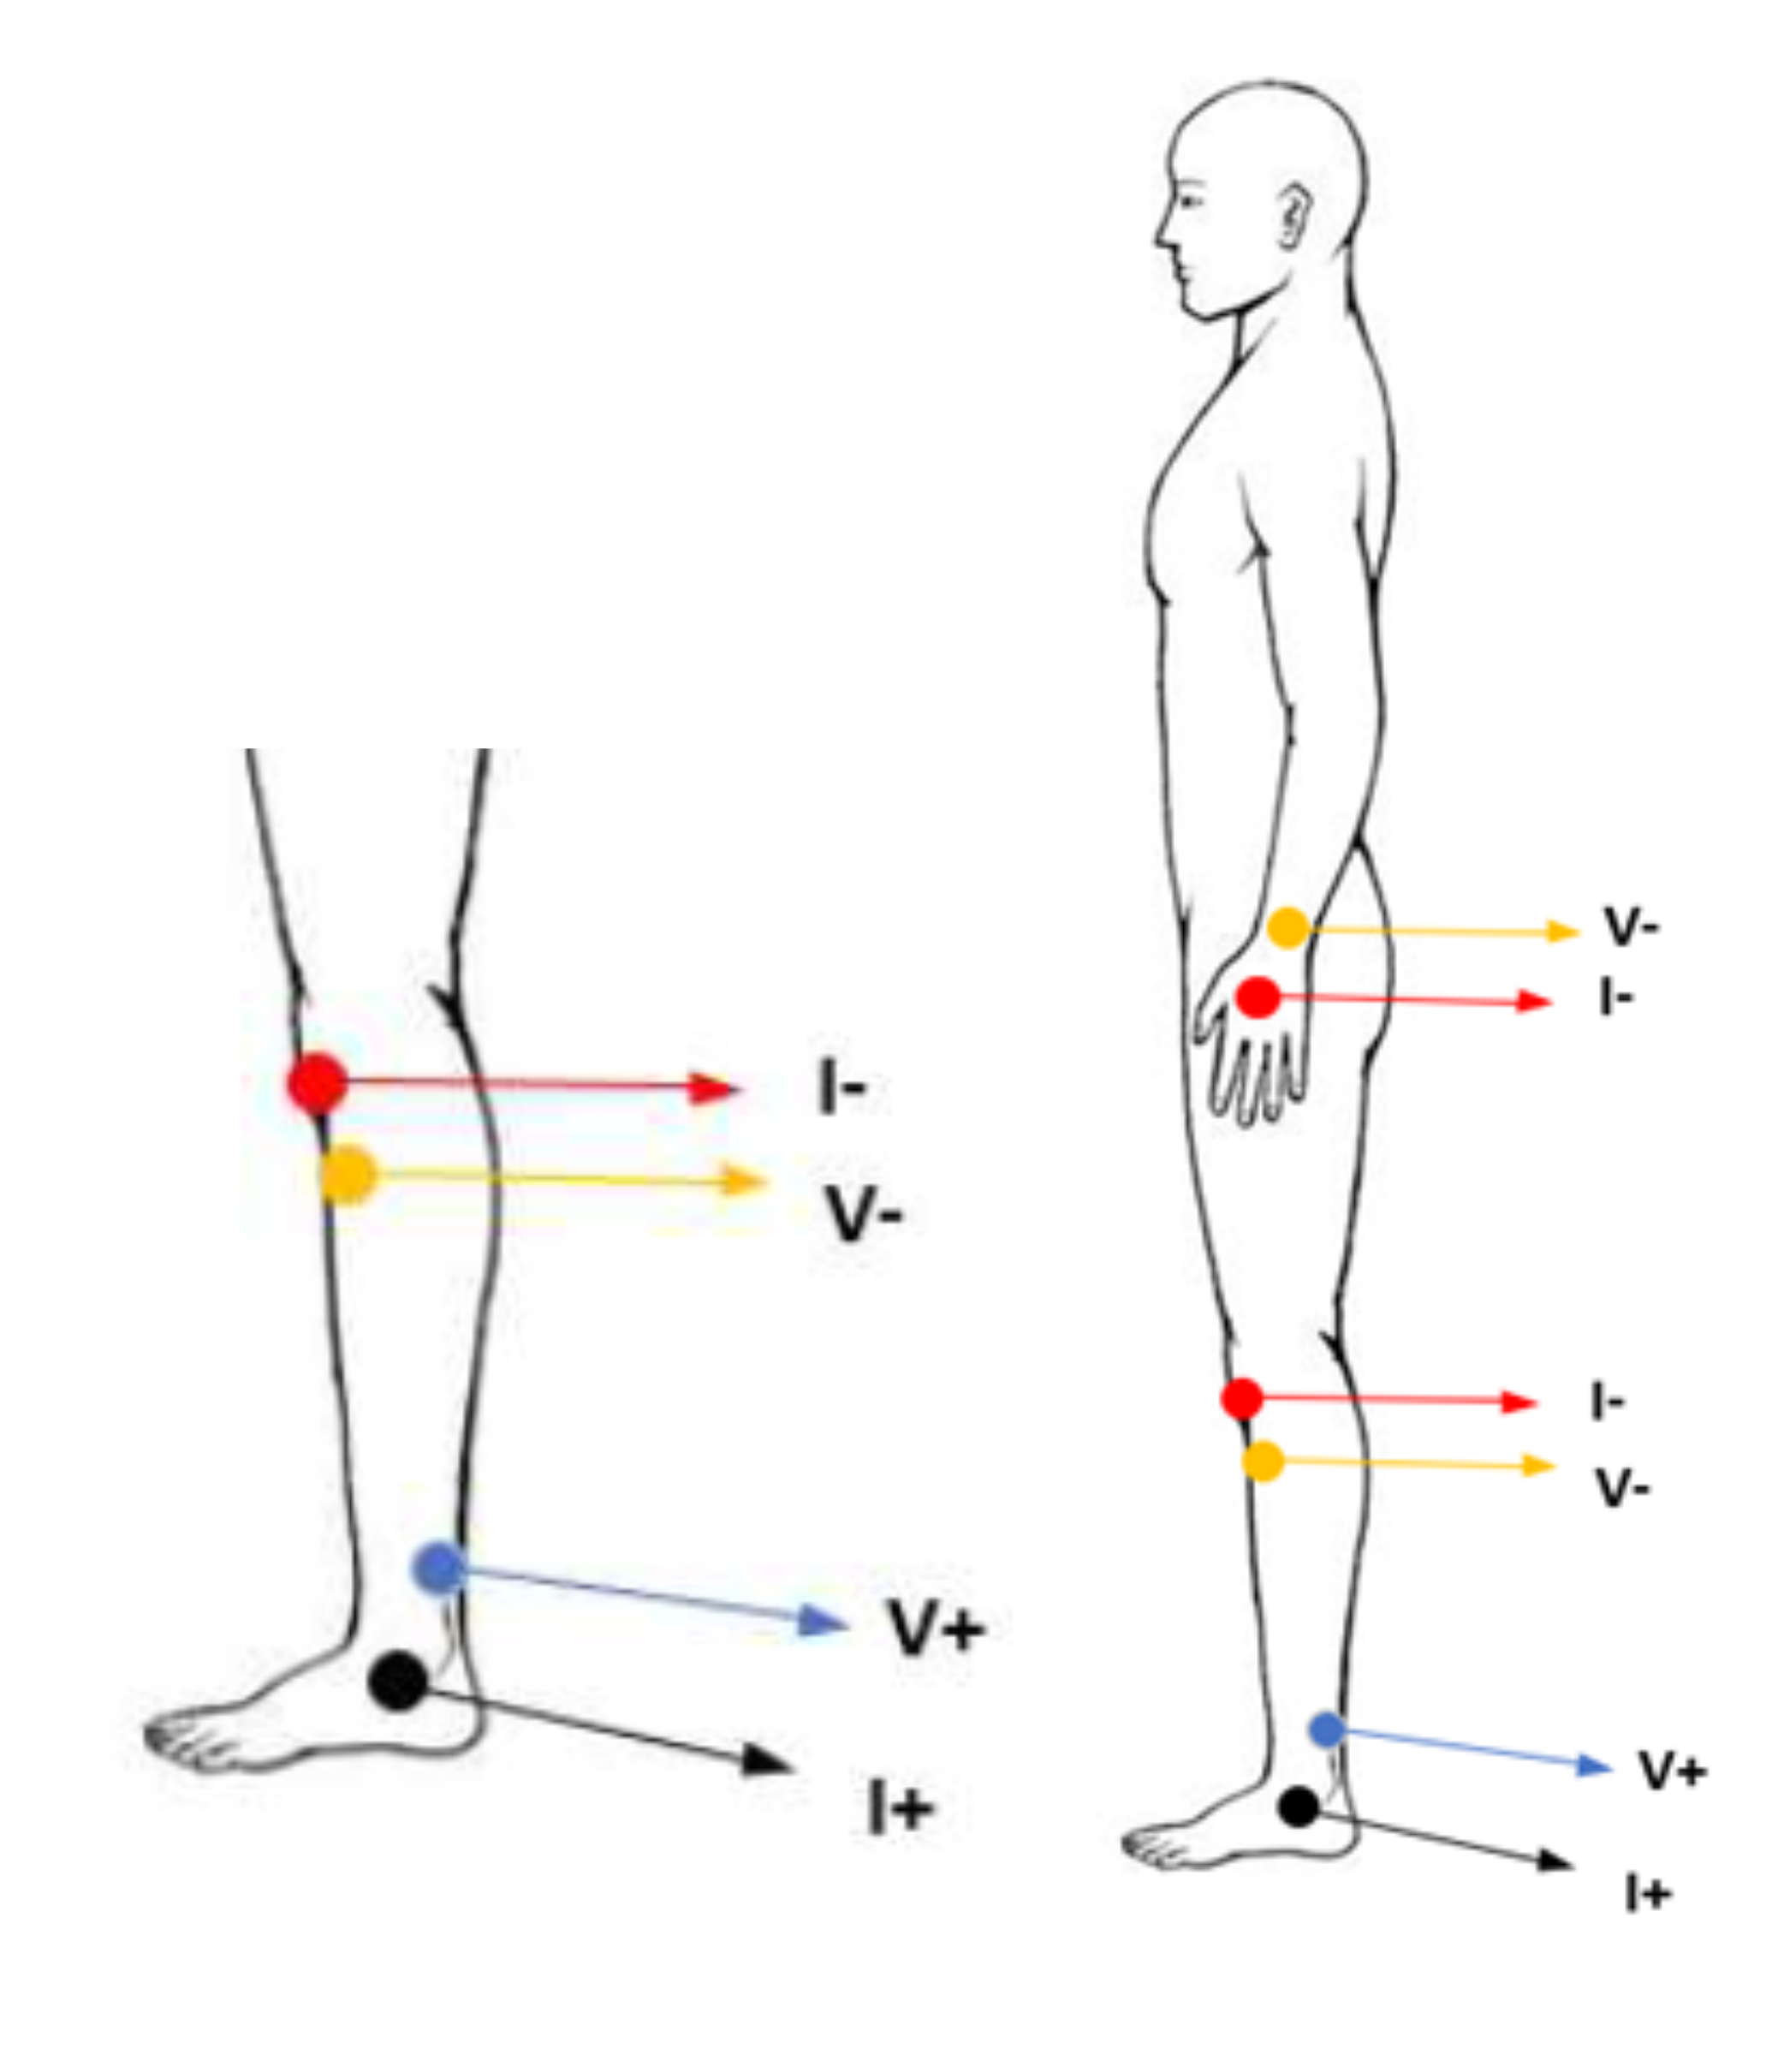
\includegraphics[width=0.65\textwidth]{Figures/postavljanje_elektroda.png} 
    \caption{Postavljanje elektroda na ispitanika \cite{Piper2023}}
    \label{slk:postavljanje_elektroda}
\end{figure}

\section{Analiza podataka}

Softver BioIMP, ImpediMed Inc., korišten je za generiranje automatskih granica iz sirovih 
vrijednosti otpora i reaktancije izmjerenih uređajem SFB7. 
Točke podataka koje su odstupale više od 1\% od izračunate krivulje isključene 
su iz izračuna vrijednosti $R_{0}$ i $R_{\infty}$ \cite{Piper2023}. 
Te vrijednosti uzimaju se kao x-presjeci u Cole-Cole dijagramu (negativna reaktancija vs. otpor) 
i koriste se za izračun volumena tekućine. 
U svakoj iteraciji, procijenjene vrijednosti $R_{0}$ i $R_{\infty}$ dobivene tekstilnim elektrodama uspoređene
su s vrijednostima zlatnog standarda gel elektroda koristeći korelacijsku analizu i korijen 
srednje kvadratne pogreške (RMSE) između dvaju mjerenja \cite{Piper2023}.

Također, prije početka mjernog procesa, izmjereni su određeni segmenti tijela (Tablica \ref{tab:segmenti_tijela}) i 
prikupljeni su demografski podaci ispitanika (Tablica \ref{tab:opci_podaci}), 
koji su korišteni u jednadžbama \cite{Sanchez2013}, \cite{Delano2022} za procjenu volumena tekućine.


\begin{table}[H]
\centering
\begin{tblr}{
    width=1\linewidth,
    cells={valign=m,halign=c},
    row{1}={bg=lightgray,font=\bfseries,rowsep=8pt},
    cell{1}{1} = {c = 3}{halign = c},
    cell{1}{4} = {r = 2}{valign = m},
    hlines,
    vlines
}
    \hline
    Opseg &  &  & Razmak elektroda \\ [0.5ex] 
    \hline
    Gležanj & List & Koljeno &  \\ [0.5ex] 
    \hline\hline
    23.48±1.30 & 36.92±53.46  & 34.92±2.90 & 10.07±3.09  \\
    \hline
\end{tblr}
\caption{\label{tab:segmenti_tijela}Izmjereni segmenti tijela}
\end{table}

\section{Rezultat}

U ovom istraživanju analizirani su bioimpedancijski signali tijekom plantarnih fleksija za šest sudionika. 
Mjerenja su provedena na pet različitih frekvencija (5kHz, 50kHz, 100kHz, 200kHz, i 500kHz). 
Analizirani su otpor i reaktancija, a izračunata je i razlika između početne i završne vrijednosti za svaku frekvenciju.

\begin{figure}[htb]
    \centering
    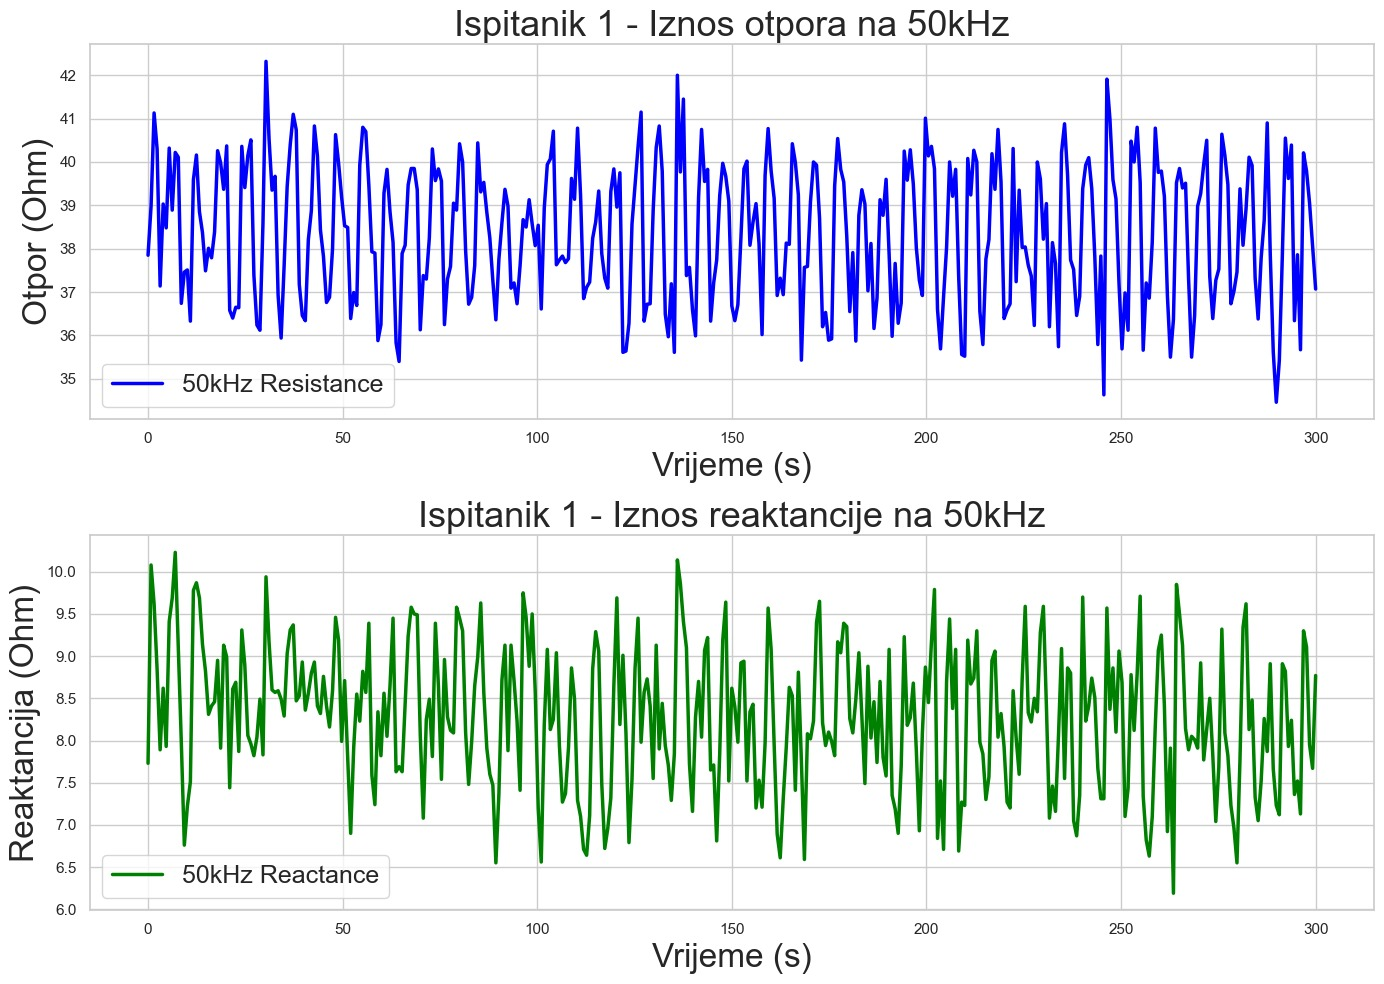
\includegraphics[width=0.65\textwidth]{Figures/otpor_i_reaktancija.jpeg} 
    \caption{Ispitanik 1 - otpor i reaktancija tijekom provedenog mjerenja}
    \label{slk:otpor_i_reaktancija}
\end{figure}

Procjena broja plantarnih fleksija izvršena je detekcijom vrhova u signalu otpora na frekvenciji od 50kHz. 
Rezultati prikazani na stupčanom grafikonu (slika \ref{slk:broj_fleksija}) pokazuju broj plantarnih 
fleksija za svakog sudionika tijekom 5 minuta. 
Razlike u broju vrhova među sudionicima mogu biti povezane s individualnim razlikama u performansama i izdržljivosti.

\begin{figure}[htb]
    \centering
    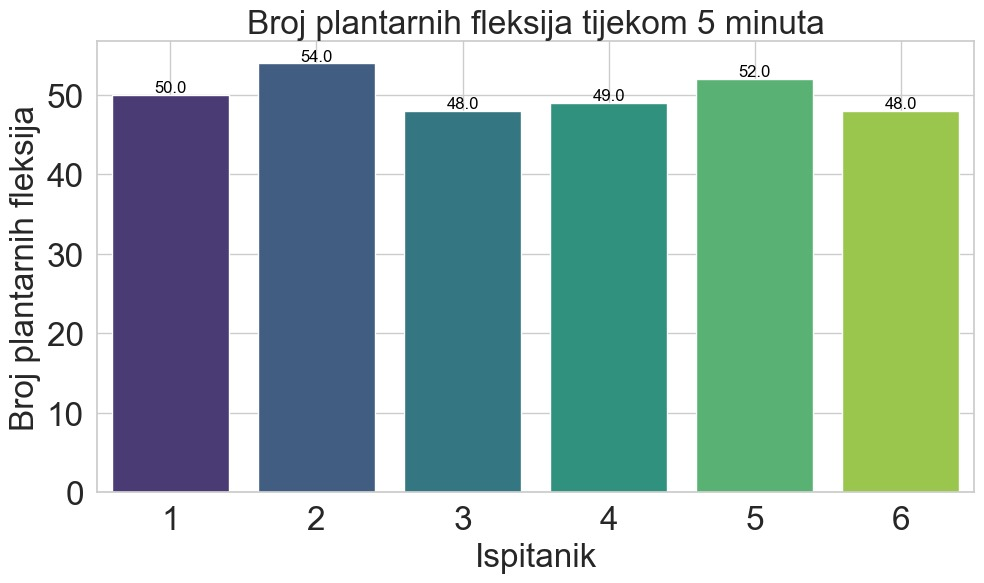
\includegraphics[width=0.65\textwidth]{Figures/broj_fleksija.jpeg} 
    \caption{Broj plantarnih fleksija tijekom 5 minuta za svakog ispitanika}
    \label{slk:broj_fleksija}
\end{figure}

Otpor predstavlja sposobnost tkiva da se suprotstavi električnoj struji. 
Tijekom vježbanja, otpor se može smanjivati zbog promjena u perfuziji mišića, 
temperature i akumulacije metabolita. U našim mjerenjima, vidimo trend smanjenja otpora tijekom vremena. 
To može biti indikacija povećane perfuzije mišića i bolju cirkulaciju krvi, 
što omogućuje bolji prijenos kisika i hranjivih tvari te uklanjanje metabolita kao što je laktat. 
Smanjenje otpora također može biti povezano s redistribucijom tekućine iz 
međustaničnog u unutarstanični prostor zbog osmolarnosti i pritiska tijekom mišićne aktivnosti.

\begin{figure}[htb]
    \centering
    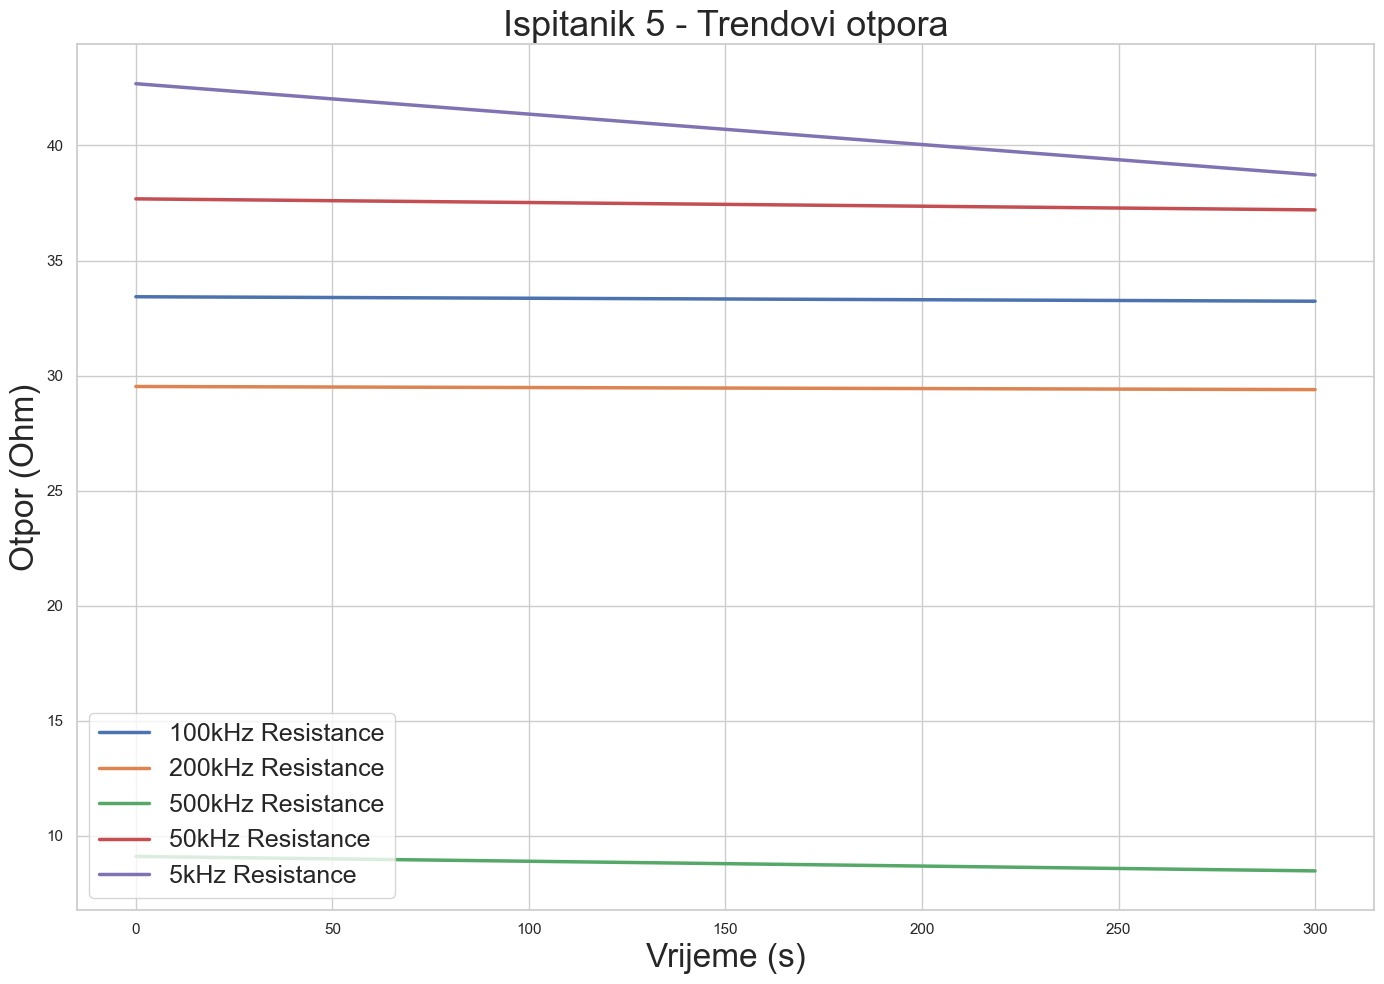
\includegraphics[width=0.65\textwidth]{Figures/trend.jpeg} 
    \caption{Ispitanik 5 - trendovi otpora}
    \label{slk:trend}
\end{figure}

Reaktancija odražava kapacitivni otpor tkiva, koji je povezan s promjenama u staničnoj membrani i strukturi tkiva. 
Tijekom vježbanja, reaktancija može opadati zbog povećanja krvnog protoka i promjena u hidriranosti tkiva. 
U našim mjerenjima, trend smanjenja reaktancije tijekom vremena može ukazivati na povećanje 
vaskularnog volumena u mišićima zbog vazodilatacije i povećanog krvnog protoka. 
Također, smanjenje reaktancije može biti povezano s promjenama u staničnoj membrani uslijed mišićne kontrakcije i opuštanja.

Promjene u otporu i reaktanciji mogu pružiti važne informacije o 
fiziološkim procesima koji se odvijaju tijekom vježbanja. 
Smanjenje otpora može biti indikator povećane perfuzije i bolje cirkulacije, 
što može biti korisno za praćenje performansi sportaša i planiranje oporavka. 
Smanjenje reaktancije može ukazivati na poboljšanu perfuziju i hidriranost mišića, 
što je važno za procjenu učinkovitosti treninga i oporavka.

Deskriptivna statistika (srednja vrijednost ± standardna devijacija) 
za razliku u otporu i reaktanciji prikazana je u tablici \ref{tab:deskriptivna_statistika}. 
Rezultati pokazuju da postoji varijabilnost u promjenama otpora i reaktancije među različitim frekvencijama. 
Veće promjene su primijećene na višim frekvencijama (50kHz i 500kHz), 
što može ukazivati na veće promjene u bioelektričnoj aktivnosti mišića i tekućine tijekom vježbanja.

\begin{table}[H]
\centering
\begin{tblr}{
    width=1\linewidth,
    cells={valign=m,halign=c},
    row{1}={bg=lightgray,font=\bfseries,rowsep=8pt},
    column{1}={2.4cm},
    column{2}={2.7cm},
    column{3}={2.7cm},
    column{4}={2.7cm},
    column{5}={2.7cm},
    hlines,
    vlines
}
    \hline
    Frekvencija (kHz) & Srednja vrijednost razlike otpora ($\Omega$) & Standardna devijacija razlike otpora ($\Omega$) & Srednja vrijednost razlike reaktancije ($\Omega$) & Standardna devijacija razlike reaktancije ($\Omega$) \\ [0.5ex] 
    \hline\hline
    5 & 0.5  & 0.1 & 0.4 & 0.05 \\
    50 & 1.2  & 0.2 & 1.1 & 0.18 \\
    100 & 0.8  & 0.15 & 0.75 & 0.12 \\
    200 & 0.6  & 0.1 & 0.55 & 0.08 \\
    500 & 1.1  & 0.25 & 1.0 & 0.2 \\
    \hline
\end{tblr}
\caption{\label{tab:deskriptivna_statistika}Deskriptivna statistika}
\end{table}

\end{document}